\documentclass[11pt]{beamer}

\mode<presentation>
{
 \usetheme{Boadilla}
\pagestyle{empty}

\setbeamerfont*{frametitle}{size=\normalsize,series=\bfseries}
\setbeamerfont*{block}{size=\normalsize,series=\bfseries}
%\setbeamertemplate{blocks}[rounded][shadow=true]
}

\definecolor{links}{HTML}{2A1B81}
\hypersetup{colorlinks,linkcolor=,urlcolor=links}


\usepackage[pdf]{pstricks}
\usepackage{pst-sigsys}



\definecolor{darkblue}{rgb}{0.0, 0.0, 0.40}
\setbeamercolor{title}{fg=darkblue}
\setbeamercolor{frametitle}{fg=darkblue}
\definecolor{darkgreen}{rgb}{0.0, 0.4, 0.0}

\usepackage{bbm}



\def\nn{\nonumber}
\def\xt{x(t)}
\def\xn{x[n]}
\def\xeven{x_{\text{even}}}
\def\xodd{x_{\text{odd}}}
\def\e{\text{e}}

%\newcommand{\re}[1]{\mathcal{R}_{#1}}
%\newcommand{\im}[1]{\mathcal{I}_{#1}}

\newcommand{\re}[1]{r_{#1}}
\newcommand{\im}[1]{i_{#1}}

\newcommand{\fs}[2]{#2}

\title[]{Complex Exponential Signals}
\author[\textcolor{blue}{Systems and Circuits}]{\textcolor{darkblue}{Pablo M. Olmos} (olmos@tsc.uc3m.es)\\ \textcolor{darkblue}{Emilio Parrado} (emipar@tsc.uc3m.es)}
\institute{\textcolor{white}{UC3M}}

\AtBeginSection[]
{
  \begin{frame}<beamer>{Index}
    \tableofcontents[currentsection,currentsubsection]
  \end{frame}
}

\AtBeginSubsection[]
{
  \begin{frame}<beamer>{Index}
    \tableofcontents[currentsection,currentsubsection]
  \end{frame}
}

\begin{document}

\frame{
\titlepage
\thispagestyle{empty}
\begin{center}

\includegraphics[scale=0.055]{Figures/uc3m-logo2.pdf}
\end{center}
}



\frame{
\begin{align*}
a=\re{a}+j\im{a}
\end{align*}

\begin{columns}
\begin{column}{0.5\textwidth}
\begin{figure}
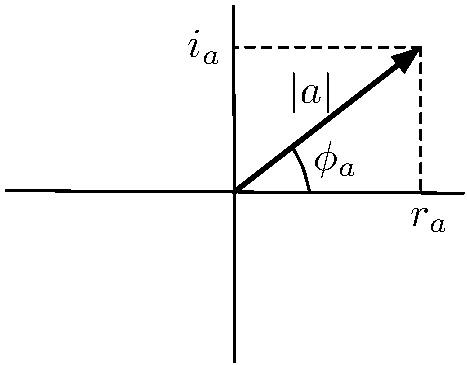
\includegraphics[scale=0.6]{Figures/Signal70.pdf}
\end{figure}
\end{column}
\begin{column}{0.5\textwidth}
\begin{itemize}
\item $|a|^2=\re{a}^2+\im{a}^2$
\item $\phi_a\;\;=\arctan\left(\frac{\im{a}}{\re{a}}\right)$
\end{itemize}
\begin{itemize}
\item $\re{a}=|a|\cos(\phi_a)$
\item $\im{a}\;=|a|\sin(\phi_a)$
\end{itemize}
\end{column}
\end{columns}

\begin{block}{Using Euler's formula}
\begin{align*}
\e^{\left(\re{a}+j\im{a}\right)}=\e^{\re{a}} ~\e^{j\im{a}}=\e^{\re{a}}  \Big( \cos(\re{a})+j\sin(\im{a}) \Big)
\end{align*}
\end{block}

}

\section{Continuous-time Complex Exponential  Signals: $x(t)=a\e^{bt}$}

\frame{
\frametitle{Complex exponential signals}
\begin{align}\nn
x(t)=a\e^{bt},
\end{align}
where $a$ and $b$ are complex numbers:
\begin{align}\nn
&a=|a|\e^{j\phi_a}=\re{a}+j\im{a}\\\nn
&b=|b|\e^{j\phi_b}=\re{b}+j\im{b}
\end{align}
}


\subsection{$a$ and $b$ are real}

\frame{
\frametitle{$x(t)=a\e^{b t}$ with  $a,b\in\mathbb{R}$}
For instance, assume $a=3$...
\begin{figure}
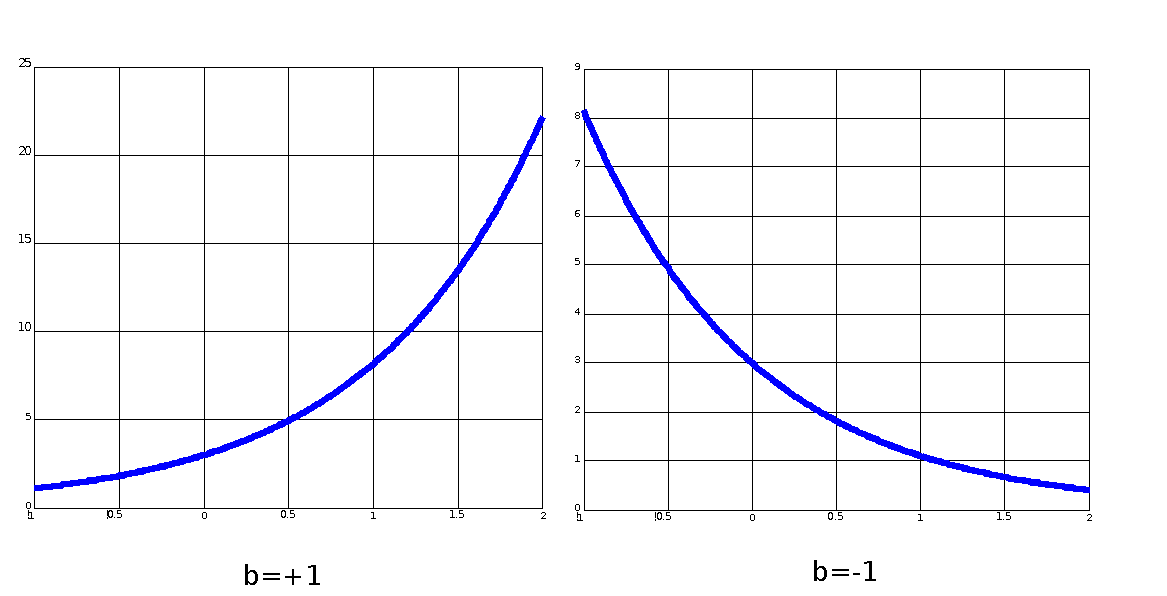
\includegraphics[scale=0.4]{Figures/Signal72.pdf}
\end{figure}
}

\subsection{$b$ is a pure imaginary number}

\frame{
\frametitle{$x(t)=a\e^{b t}$ with  $b=j\omega$} 
\begin{block}{a is real: $a\in \mathbb{R}$.}
\begin{align}\nn
x(t)=a\e^{j\omega t}=a\cos(\omega t)+ja\sin(\omega t)
\end{align}

Both the real and imaginary parts of $x(t)$ are periodic with period $T=\frac{2\pi}{\omega}$. $\omega$ is the angular frequency (radians/secod).
\end{block}

\begin{alertblock}{a is complex: $a=\re{a}+j\im{a}=|a|\e^{j\phi_a}$.}
\begin{align}\nn
x(t)=|a|\e^{j(\omega t+\phi_a)}=|a|\cos(\omega t+\phi_a)+j|a|\sin(\omega t+\phi_a)
\end{align}

Both the real and imaginary parts of $x(t)$ are periodic with period $T=\frac{2\pi}{\omega}$.
\end{alertblock}


}

\frame{
\begin{figure}
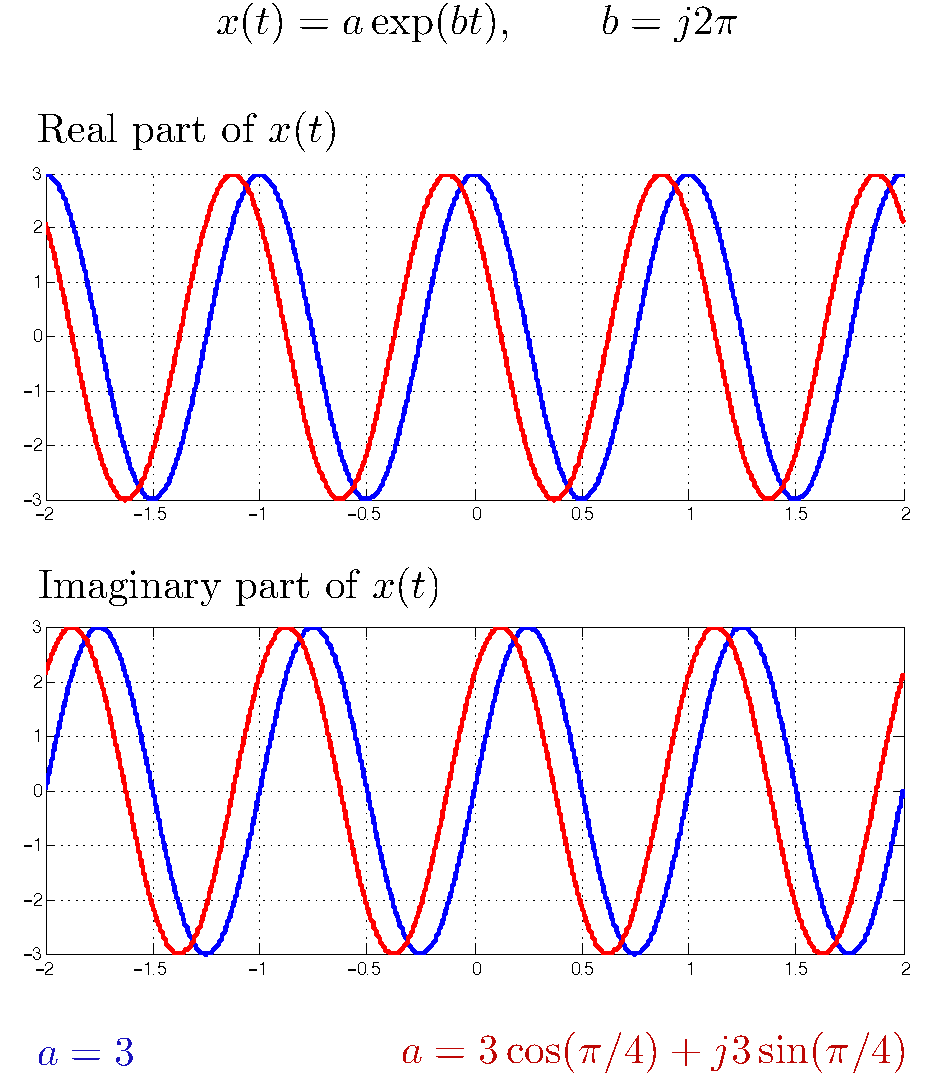
\includegraphics[scale=0.45]{Figures/Signal56.pdf}
\end{figure}
}

\subsection{$a$ and $b$ are complex}

\frame{
\frametitle{$x(t)=a\e^{b t}$ with  $a=|a|\e^{j\phi_a}$ and $b=r+j\omega$}

\begin{block}{}
\begin{align}\nn
x(t)&=|a|\e^{rt}\e^{j(\omega t+\phi_a)}\\\nn
&=|a|\e^{rt}\cos(\omega t+\phi_a)+j|a|\e^{rt}\sin(\omega t+\phi_a)
\end{align}
\end{block}

\begin{alertblock}{}
The real and imaginary parts of $x(t)$ are NOT periodic functions anymore.
\end{alertblock}
}

\frame{
\begin{figure}
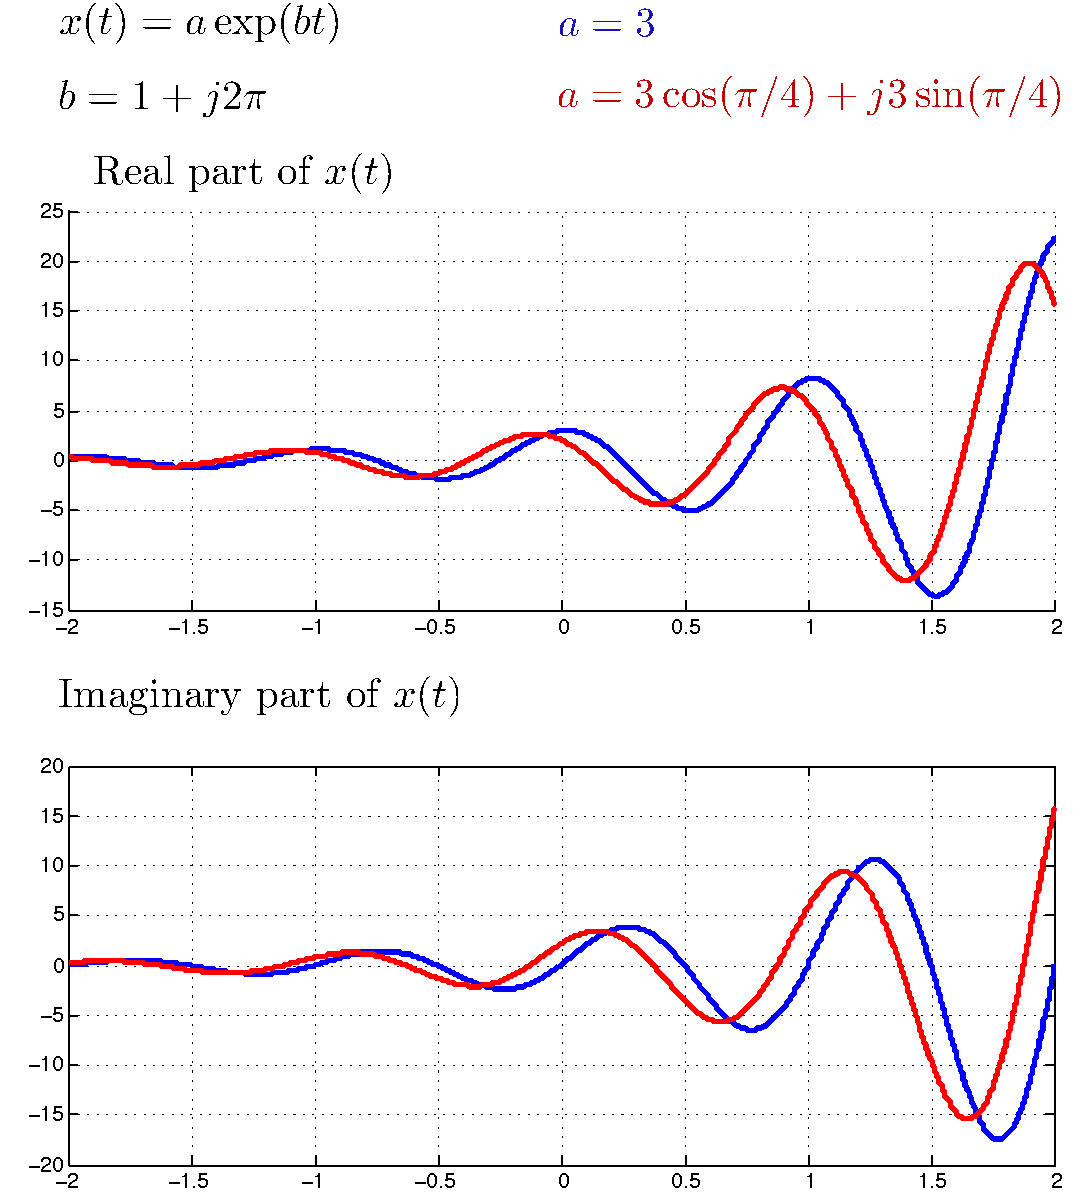
\includegraphics[scale=0.4]{Figures/Signal57.pdf}
\end{figure}
}

\frame{
\begin{figure}
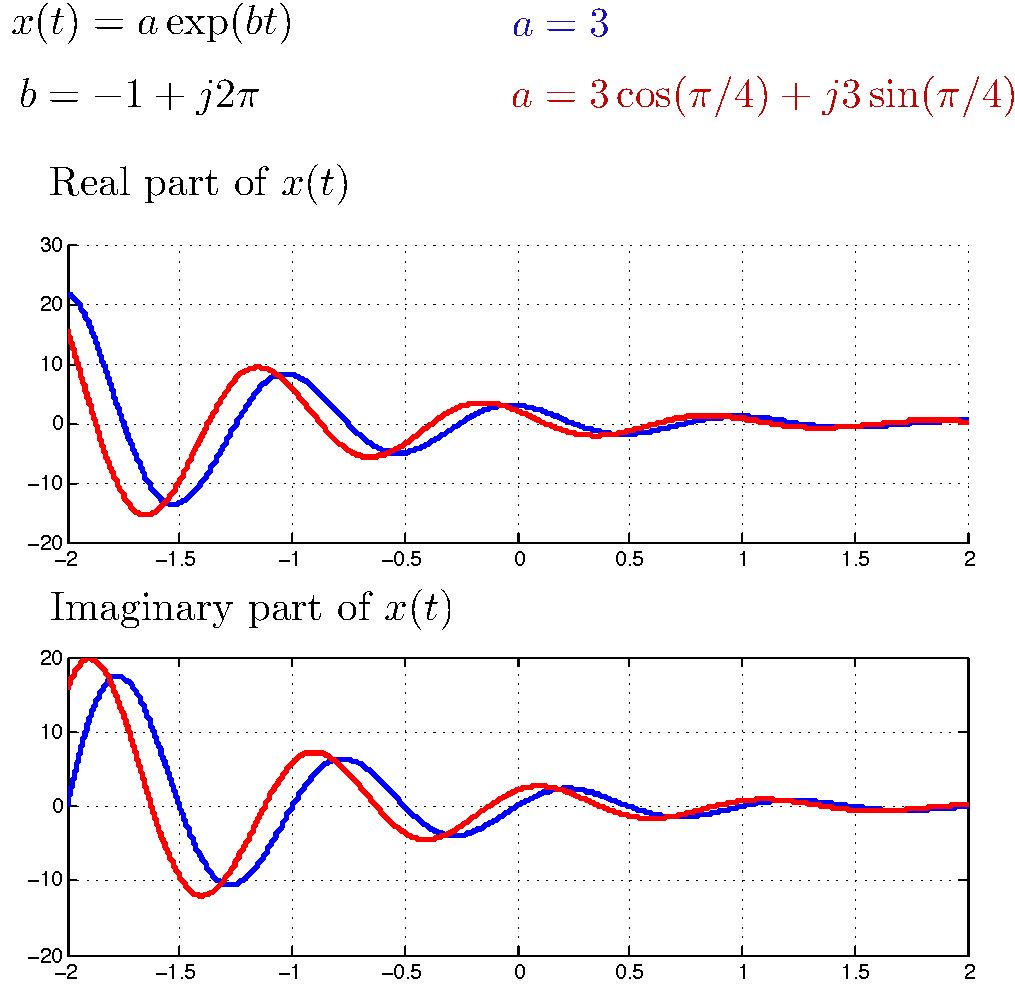
\includegraphics[scale=0.45]{Figures/Signal59.pdf}
\end{figure}
}


\section{Discrete-time Complex Exponential Signals: $x[n]=a\e^{bn}$}

\frame{
\frametitle{Discrete-time complex exponential signal}
\begin{align}\nn
x[n]=a\e^{bn},
\end{align}
where $a$ and $b$ are complex numbers:
\begin{align}\nn
&a=|a|\e^{j\phi_a}=\re{a}+j\im{a}\\\nn
&b=|b|\e^{j\phi_b}=\re{b}+j\im{b}
\end{align}
}

%\subsection{$b$ is a pure imaginary number}

\frame{
\frametitle{$x[n]=a\e^{b n}$ with $a=|a|\e^{j\phi_a}$ and $b=j\Omega$}

\begin{block}{}
\begin{align}\nn
x[n]=|a|\e^{j(\Omega n+\phi_a)}=|a|\cos(\Omega n+\phi_a)+j|a|\sin(\Omega n+\phi_a)
\end{align}
\end{block}

\begin{alertblock}{}
$x[n]$ is periodic if there exist $N\in\mathbb{Z}$ such that $\Omega N$  is a multiple of $2\pi$. 
\end{alertblock}

\begin{exampleblock}{}
\begin{itemize}
\item $x(t)=a\e^{j\omega t}$ is always periodic with period $T=2\pi/\omega$.
\item $x[n]=a\e^{j\Omega n}$ is only periodic if $\frac{2\pi}{\Omega}$ is a rational number.
\end{itemize}
\end{exampleblock}

%Therefore, the periodicity condition is 
%\begin{align}\nn
%\frac{2\pi}{\Omega}=\frac{a}{b} \text{ (Rational Number)  },
%\end{align}
%where $a,b\in\mathbb{Z}$.

}

%\frame{
%\frametitle{Continous-time and discrete-time complex exponential signal}
%
%\begin{itemize}
%\item $x(t)=C\e^{j\omega t}$ is always periodic with period $T=2\pi/\omega$.
%\item $x[n]=C\e^{j\Omega n}$ is only periodic if $\frac{2\pi}{\Omega}$ is a rational number.
%\end{itemize}
%}

\frame{
\begin{exampleblock}{Periodicity in the frequency domain \textbf{ (Discrete case!) }}
\begin{align}\nn
&x[n]=a\e^{j\Omega n}\\\nn
&y[n]=a\e^{j(\Omega+2\pi k)n}=a\e^{\Omega n}\e^{j2\pi k}=a\e^{\Omega n}=x[n] \qquad \forall n \text{ if  } k\in\mathbb{Z} 
\end{align}
\end{exampleblock}

\begin{alertblock}{}
The continuous-time complex exponential $ x(t)=a\e^{j\omega t}$ is NOT periodic in the frequency domain!.
\end{alertblock}

}

\frame{
\frametitle{$x[n]=a\e^{b n}$ with $a=|a|\e^{j\phi_a}$ $b=r+j\Omega$}

\begin{block}{}
\begin{align}\nn
x[n]&=|a|\e^{rn}\e^{j(\Omega n+\phi_a)}\\\nn
&=|a|\e^{rn}\cos(\Omega n+\phi_a)+j|a|\e^{rn}\sin(\Omega n+\phi_a)
\end{align}
\end{block}

\begin{alertblock}{}
$x[n]$ is not periodic.
\end{alertblock}
}


\end{document}
